

\documentclass[12pt]{article}
\usepackage{graphicx}

\begin{document}


\section{UI Prototyping}

\paragraph{Outline}
User Interface Prototyping is a technique of developing mock-up diagrams for your future mobile application. After discussing with all team members, we designed all these mock ups for our future mobile app which would deliver users with a best UI interface. It would attract the users towards our application and their experience of ordering food would be great with our proposed UI design. Here are some mock-up designed diagrams which would give you an idea of our application

\begin{figure}
\centering
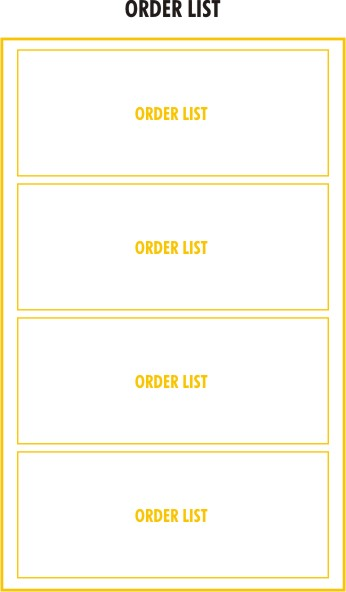
\includegraphics[scale=0.4]{milestone2/1.jpeg}
\caption{order list}

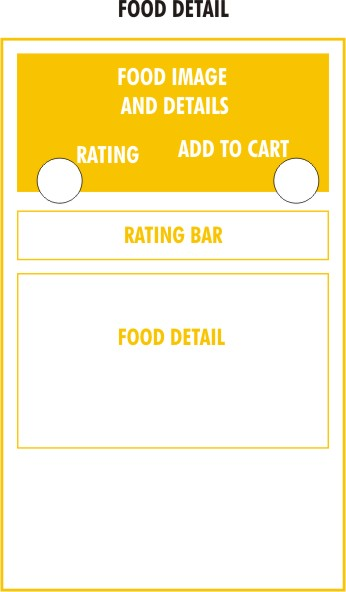
\includegraphics[scale=0.4]{milestone2/2.jpeg}
\caption{food detail}
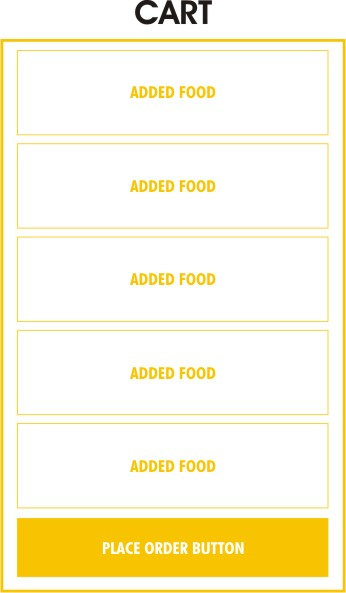
\includegraphics[scale=0.4]{milestone2/3.jpeg}
\caption{cart}

\end{figure}
\begin{figure}
\centering
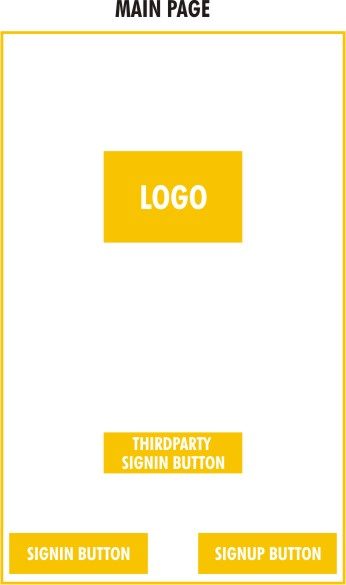
\includegraphics[scale=0.4]{milestone2/4.jpeg}
\caption{main page}
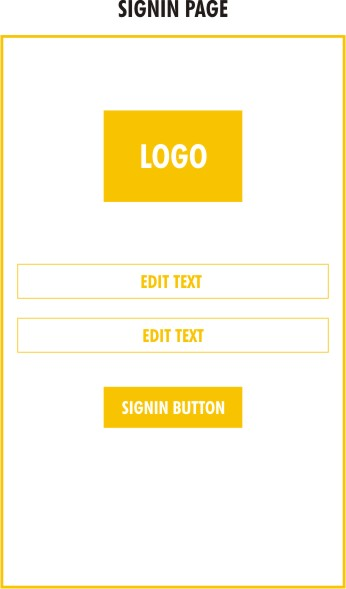
\includegraphics[scale=0.4]{milestone2/5.jpeg}
\caption{sign in page}
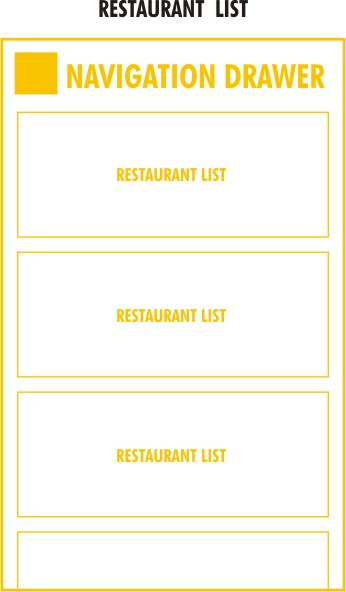
\includegraphics[scale=0.4]{milestone2/6.jpeg}
\caption{restaurant list}


\end{figure}

\begin{figure}
\centering
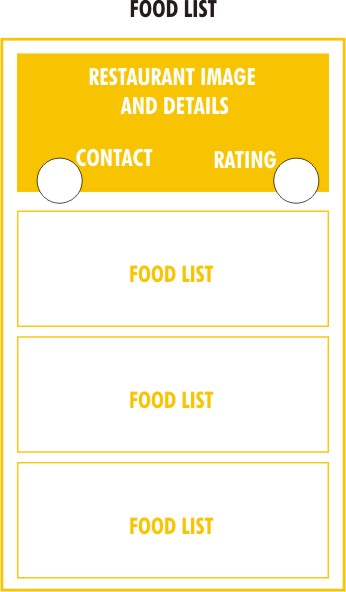
\includegraphics[scale=0.4]{milestone2/7.jpeg}
\caption{food list}
\end{figure}





































\bibliographystyle{abbrv}
\bibliography{main}

\end{document}